\documentclass[aspectratio=1610,notes,blackandwhite,mathsans,usenames,dvipsnames]{beamer}

\usepackage{amsmath}
\usepackage{amssymb}
\usepackage{graphicx}
\usepackage{fancybox}
\usepackage{booktabs}
\usepackage{multirow,multicol,pxfonts}
\usepackage{cmbright}
\usepackage{xcolor}
\usepackage{color}
\usepackage{enumitem}
\usepackage{animate}
\usepackage{changepage}
\usepackage{cmbright}

\usepackage{natbib}

%\usepackage{shellesc}
%\AtEndDocument{\ShellEscape{sleep 10; rm *.nav *.aux *.log *.out *.snm *.gz}}

\usepackage[T1]{fontenc}
\fontencoding{T1}  
\usepackage[utf8]{inputenc}


\usefonttheme{default}
\setbeamercovered{invisible}
\beamertemplatenavigationsymbolsempty

%\makeatletter
%\setbeamertemplate{footline}
%{
%  \leavevmode
%  \hbox{
%  \begin{beamercolorbox}[wd=0.97\paperwidth,ht=2.25ex,dp=2ex,right]{}
%{\color{gre} \insertframenumber{} / \inserttotalframenumber}
%  \end{beamercolorbox}}%
%}



% Plan
% 1. Bridge the gap
% + objectives and incentives: academia vs. governance institutions
% 
%2. Package features presentation
%+ feature listings
%+ workflows
%+ plots
%+ back to the mismatch
%
%3. Roadmap:
% + bsvars
% + other packages
% + training & development
 


\definecolor{whi}{HTML}{FFFFFF}
\definecolor{lig}{HTML}{09509A}

\setbeamercolor{frametitle}{fg=lig}
\AtBeginDocument{\color{lig}}
\setbeamercolor{itemize item}{fg=lig}


\begin{document}
	\fontfamily{pag}\selectfont
	\setbeamerfont{title}{family=\fontfamily{pag}\selectfont}
	\setbeamerfont{frametitle}{family=\fontfamily{pag}\selectfont}
	\setbeamerfont{framesubtitle}{family=\fontfamily{pag}\selectfont}
	
	
	
	
	
	
	{\setbeamercolor{background canvas}{bg=lig}
		\begin{frame}
			%\centering
			
			%\vspace{1cm}
			
			\textbf{\Huge\color{whi}Structural and Predictive}\\[1.3ex]
			\textbf{\Huge\color{whi}Monetary Policy Analyses}\\[1.3ex] 
			\textbf{\Huge\color{whi}Using the R packages bsvars.org}\\[20ex]
			
			\Large
			{\color{whi}Tomasz Wo\'zniak $\bullet$ University of Melbourne}
			
		\end{frame}
	}
	
	{\setbeamercolor{background canvas}{bg=lig}
		\begin{frame}
			\centering
			
			\textbf{\LARGE\color{whi}R packages for Bayesian\\ Structural Vector Autoregressions}\\
			
\includegraphics[trim=0cm 0cm 0cm 2cm, clip, scale=0.25]{hex}
		\end{frame}
	}
		
	
	
	

	{\setbeamercolor{background canvas}{bg=lig}
		\begin{frame}
			\centering
			
			\vspace{1cm}\Huge
			\textbf{{\color{whi}a case for software packages}}
			
		\end{frame}
	}	
	
	
	
	\begin{frame}{\huge objectives and incentives}
		\Large		
		
		\begin{columns}
        		\begin{column}{0.5\textwidth}
				\textbf{\Large academia}\\[1ex]
				\large
				\begin{itemize}[label=$\blacktriangleright$]
				{\color{lig}
					\item marginal contributions\\[1ex]
					\item performance excellence\\[1ex]
					\item focus on detail\\[1ex]
					\item one-point case\\[1ex]
					\item result reproducibility
				}	
				\end{itemize}
			\end{column}
			\begin{column}{0.5\textwidth}
				\textbf{\Large governance institutions}\\[1ex]
				\large
				\begin{itemize}[label=$\blacktriangleright$]
				{\color{lig}
					\item decision-making support\\[1ex]
					\item application/data driven\\ [1ex]
					\item reporting \& communication\\[1ex]
					\item broad interpretability\\[1ex]
					\item accountability
				}	
				\end{itemize}
			\end{column}
		\end{columns}
	\end{frame}
	
	
	
	
	\begin{frame}{\huge mutual benefits}
		\Large		
		\begin{itemize}[label=$\blacktriangleright$]
		{\color{lig}
			\item knowledge \& experience exchange\\[1ex]
			\item strategic synergies \\[1ex]
			\item relevance\\[1ex]
			\item publishable outputs\\[1ex]
			\item research dissemination
		}	
		\end{itemize}
	\end{frame}

	
	
	\begin{frame}{\huge a case for software packages}
		\Large
		
		\begin{itemize}[label=$\blacktriangleright$]
		{\color{lig}
			\item potential for bridging the mismatch\\[1ex]
			\item joint development benefiting from specialisations\\[1ex]
			\item respectful of parties' objectives and needs \\[1ex]
			\item strategically planned development and rollout
		}	
		\end{itemize}
	\end{frame}

	
	
	
	
	
	{\setbeamercolor{background canvas}{bg=lig}
		\begin{frame}
			\centering
			
			\vspace{1cm}\Huge
			\textbf{{\color{whi}bsvars.org features}}
			
		\end{frame}
	}	

	
	
	
	\begin{frame}{\huge bsvars.org features}
		\Large
		
		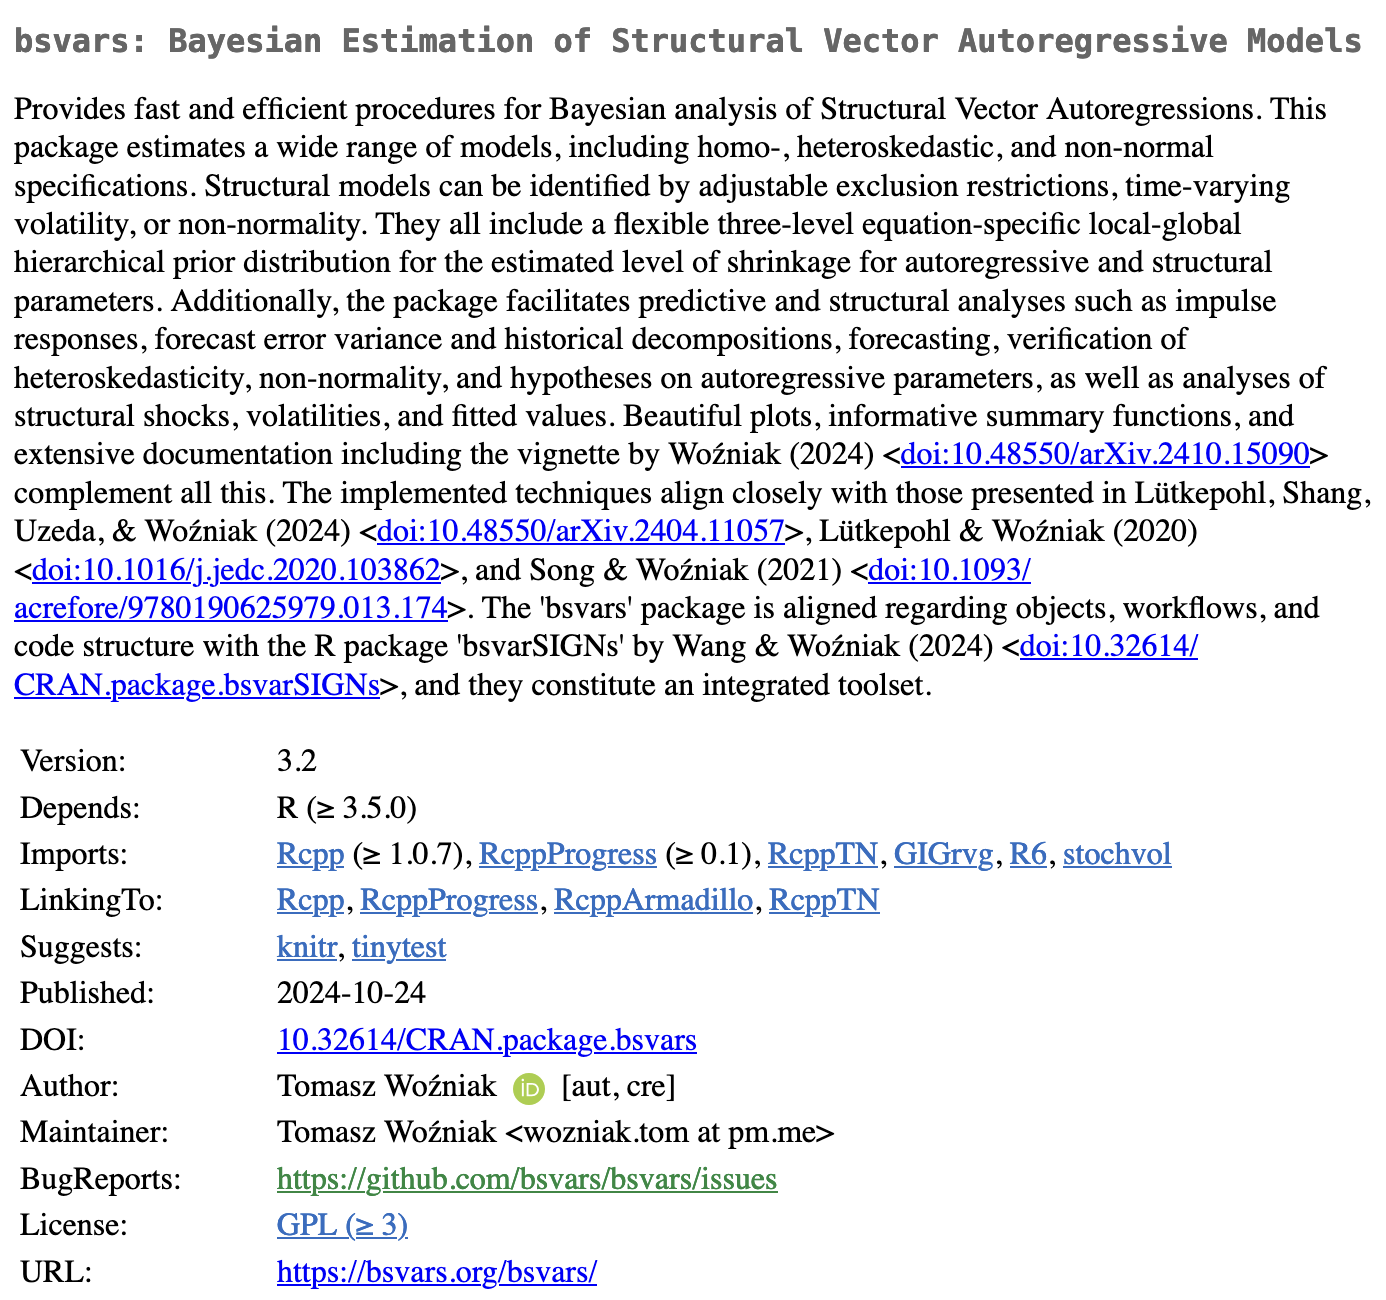
\includegraphics[scale=0.28]{bsvars_cran}
		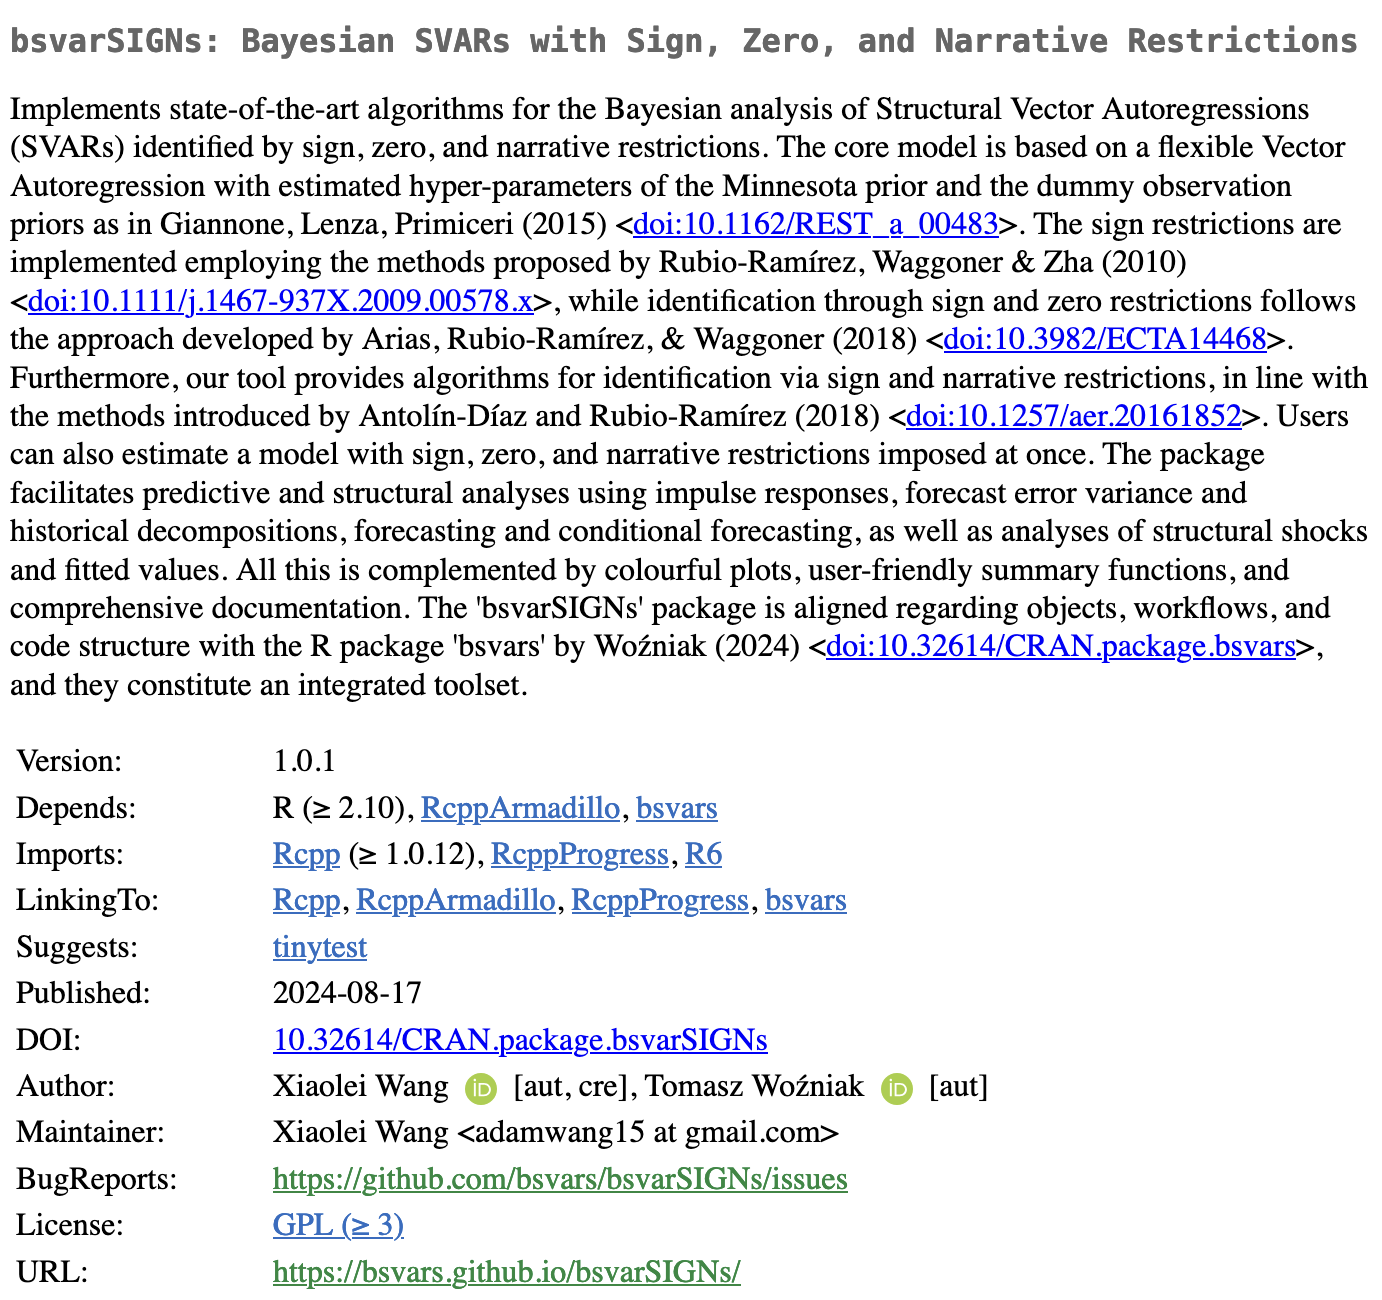
\includegraphics[scale=0.28]{bsvarSIGNs_cran}
		
	\end{frame}
	
	
	\begin{frame}{\huge bsvars.org features}
		\Large
		
		\begin{itemize}[label=$\blacktriangleright$]
		{\color{lig}
			\item Bayesian estimation of Structural VARs\\[1ex]
			\item coherent code structure, workflows, and objects\\[1ex]
			\item  excellent computational speed\\[1ex]
			\item  frontier econometric \& numerical techniques\\[1ex]
			\item  written in \textbf{C++} using \textbf{Rcpp} and \textbf{RcppArmadillo}\\[1ex]
			\item data analysis in \textbf{R}
		}	
		\end{itemize}
	\end{frame}



	\begin{frame}{\huge bsvars.org features}
		\Large
		\textbf{Structural Vector Autoregressions}
		\begin{align*}
		\text{VAR eq.:}&& \mathbf{y}_t &= \mathbf{Ax}_t + \boldsymbol\epsilon_t\\[1ex]
		\text{structural eq.:}&& \mathbf{B}_0\boldsymbol\epsilon_t &= \mathbf{u}_t \\[1ex]
		\text{structural shocks:}&& \mathbf{u}_t &\sim\mathcal{N}(\mathbf{0}, \text{diag}\left(\boldsymbol\sigma^2_t\right) ) \\
		\end{align*}
		
	\end{frame}



	

	\begin{frame}{\huge bsvars.org features}
		\Large		
		
		\begin{columns}
        		\begin{column}{0.5\textwidth}
				
\includegraphics[scale=0.35]{bsvars}\\[1ex]

				\large
				\begin{itemize}[label=$\blacktriangleright$]
				{\color{lig}
					\item based on own research\\ [1ex]
					\item exclusion restrictions\\[1ex]
					\item heteroskedasticity, and\\[1ex]
					\item non-normality\\[1ex]
					\item 5 volatility \& 3 non-normal models\\[1ex]
					\item Priors: 3-level eq-specific local-global shrinkage
				}	
				\end{itemize}
			\end{column}
			\begin{column}{0.5\textwidth}
				
\includegraphics[scale=0.35]{bsvarSIGNs}\\[1ex]
				
				\large
				\begin{itemize}[label=$\blacktriangleright$]
				{\color{lig}
					\item based on top-field papers\\ [1ex]
					\item sign restrictions\\ [1ex]
					\item sign \& zero restrictions\\[1ex]
					\item narrative restrictions\\[1ex]
					\item flexible Bayesian VAR\\[1ex]
					\item Priors: Minnesota with dummy observations and estimated shrinkage
				}	
				\end{itemize}
			\end{column}
		\end{columns}
	\end{frame}
	
	
	
	
	
	
	\begin{frame}{\huge bsvars.org features}
		\centering
		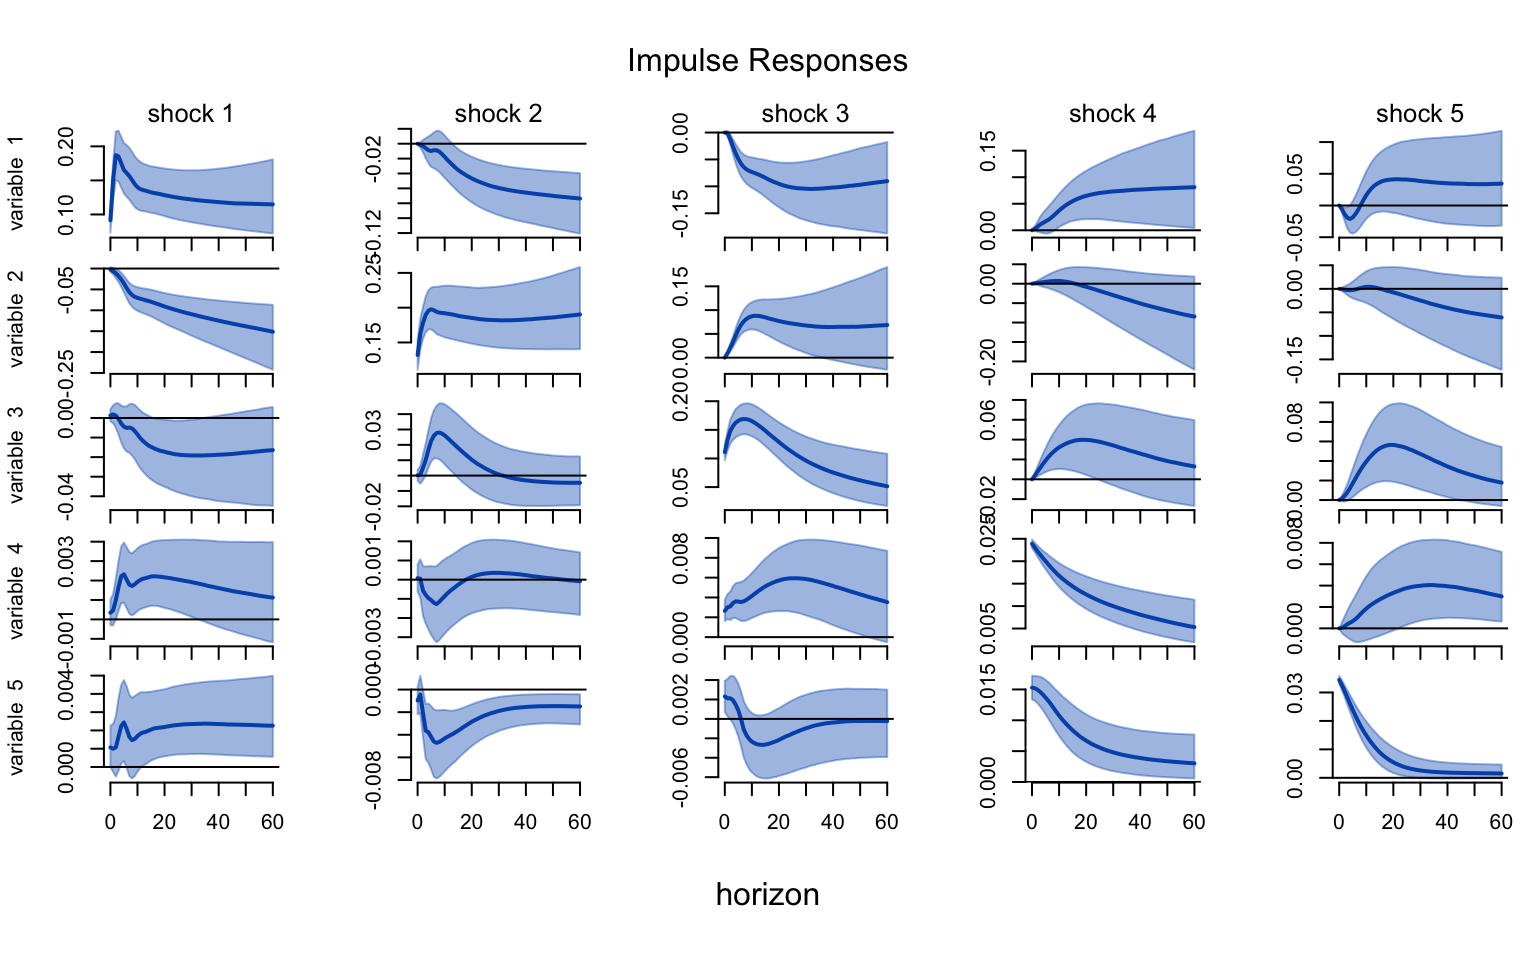
\includegraphics[scale=0.25]{bs_irf}
	\end{frame}
	
	
	
	\begin{frame}{\huge bsvars.org features}
		\centering
		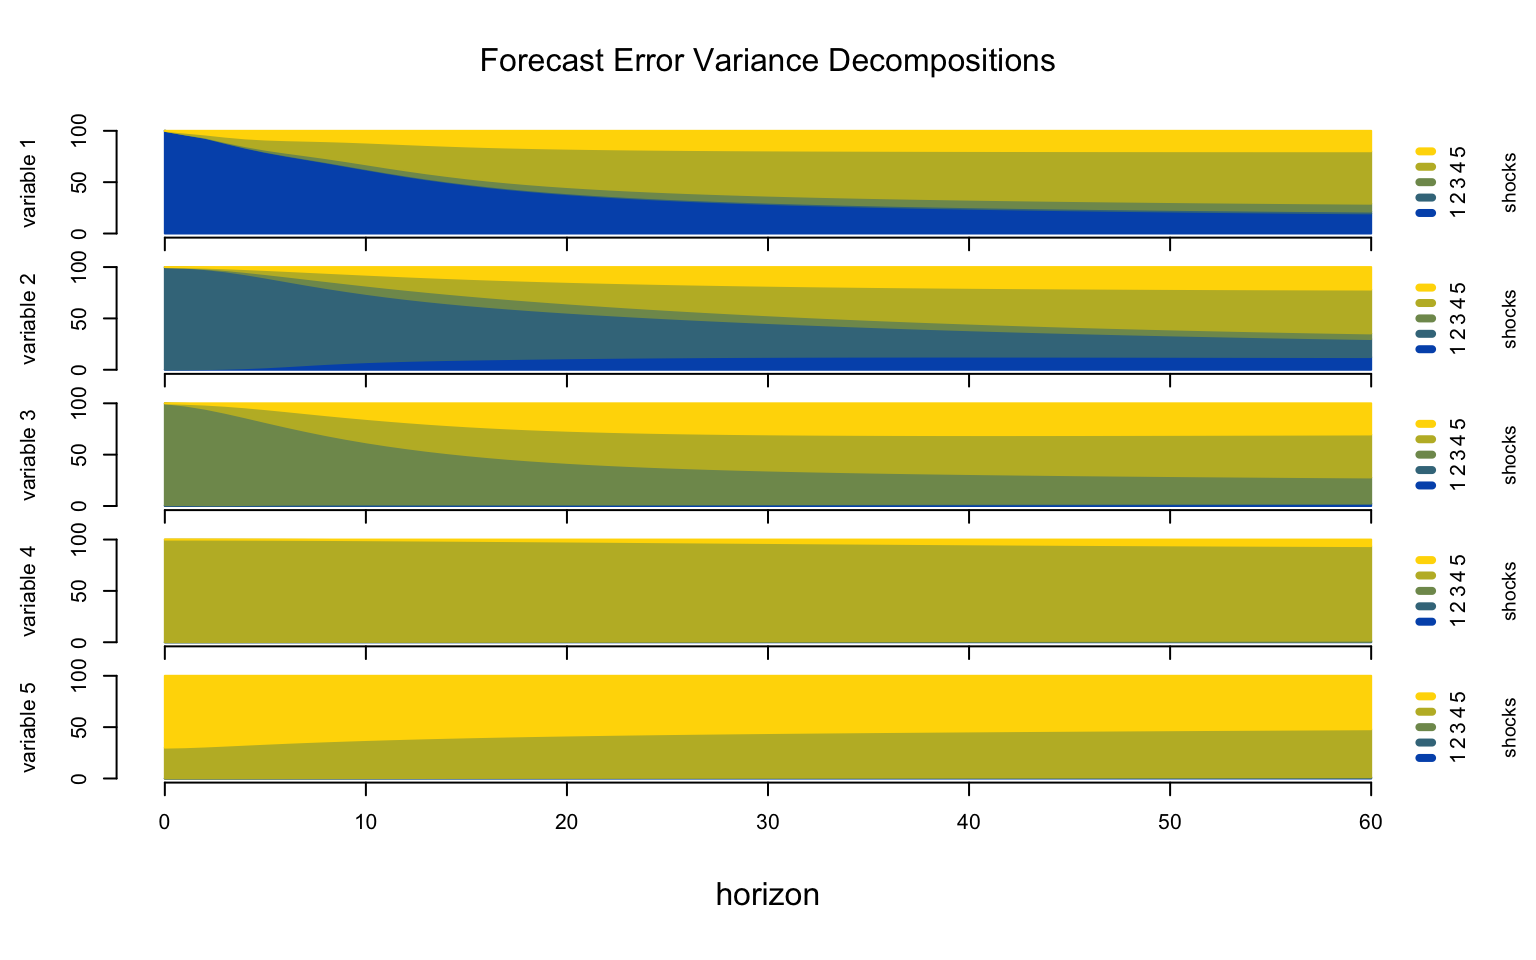
\includegraphics[scale=0.25]{bs_fevd}
	\end{frame}
	
	
	\begin{frame}{\huge bsvars.org features}
		\centering
		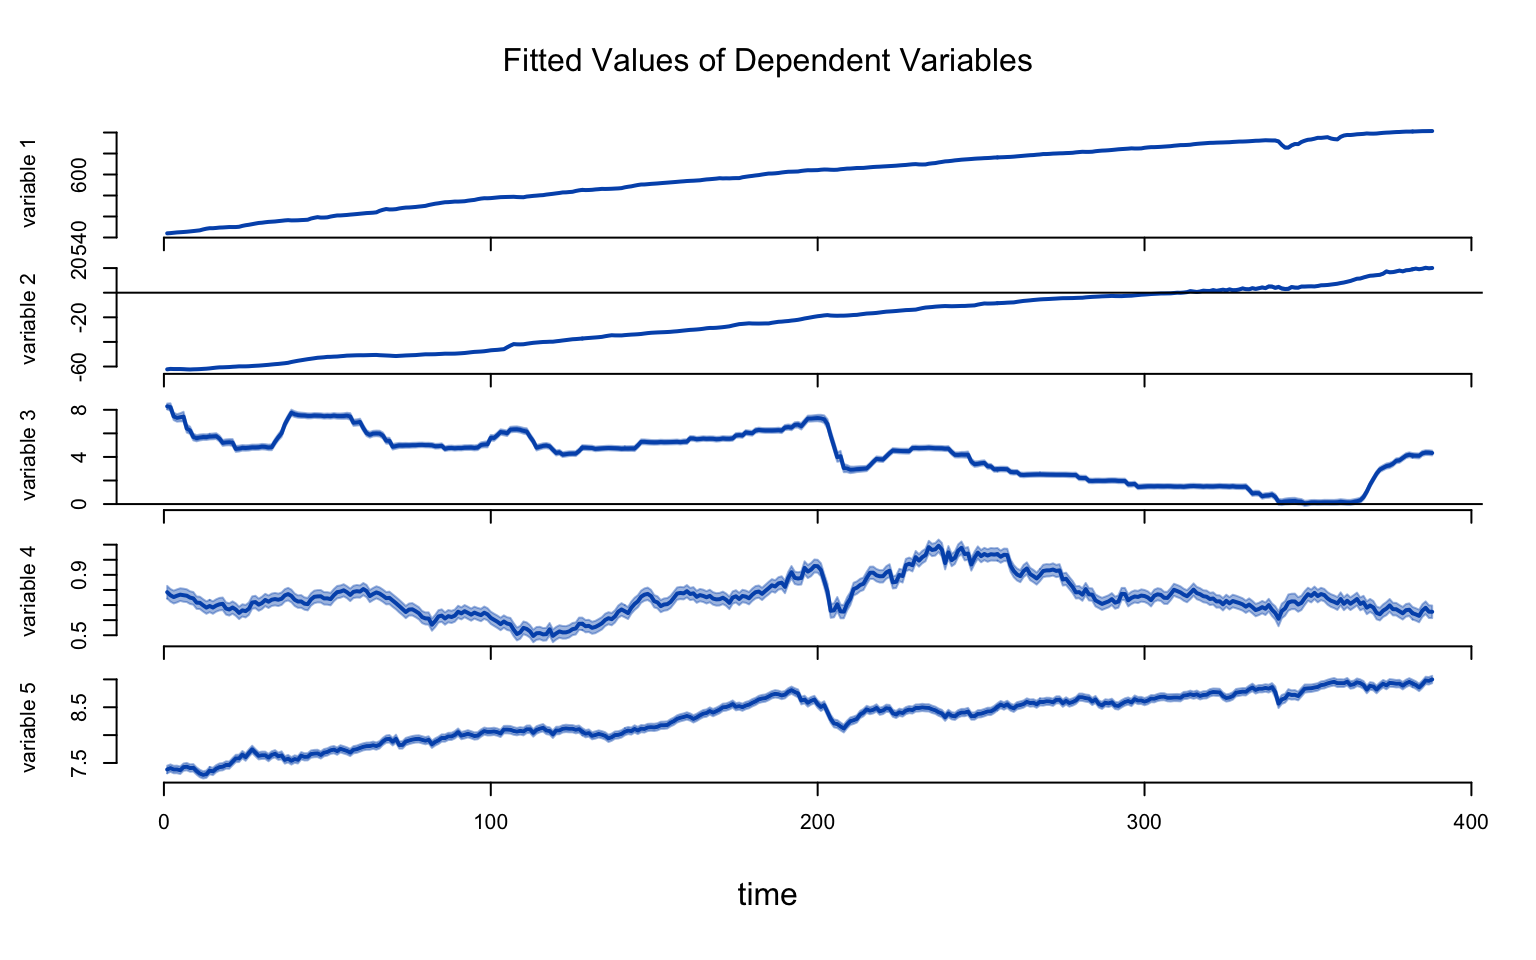
\includegraphics[scale=0.25]{bs_fit}
	\end{frame}
	
	
	\begin{frame}{\huge bsvars.org features}
		\centering
		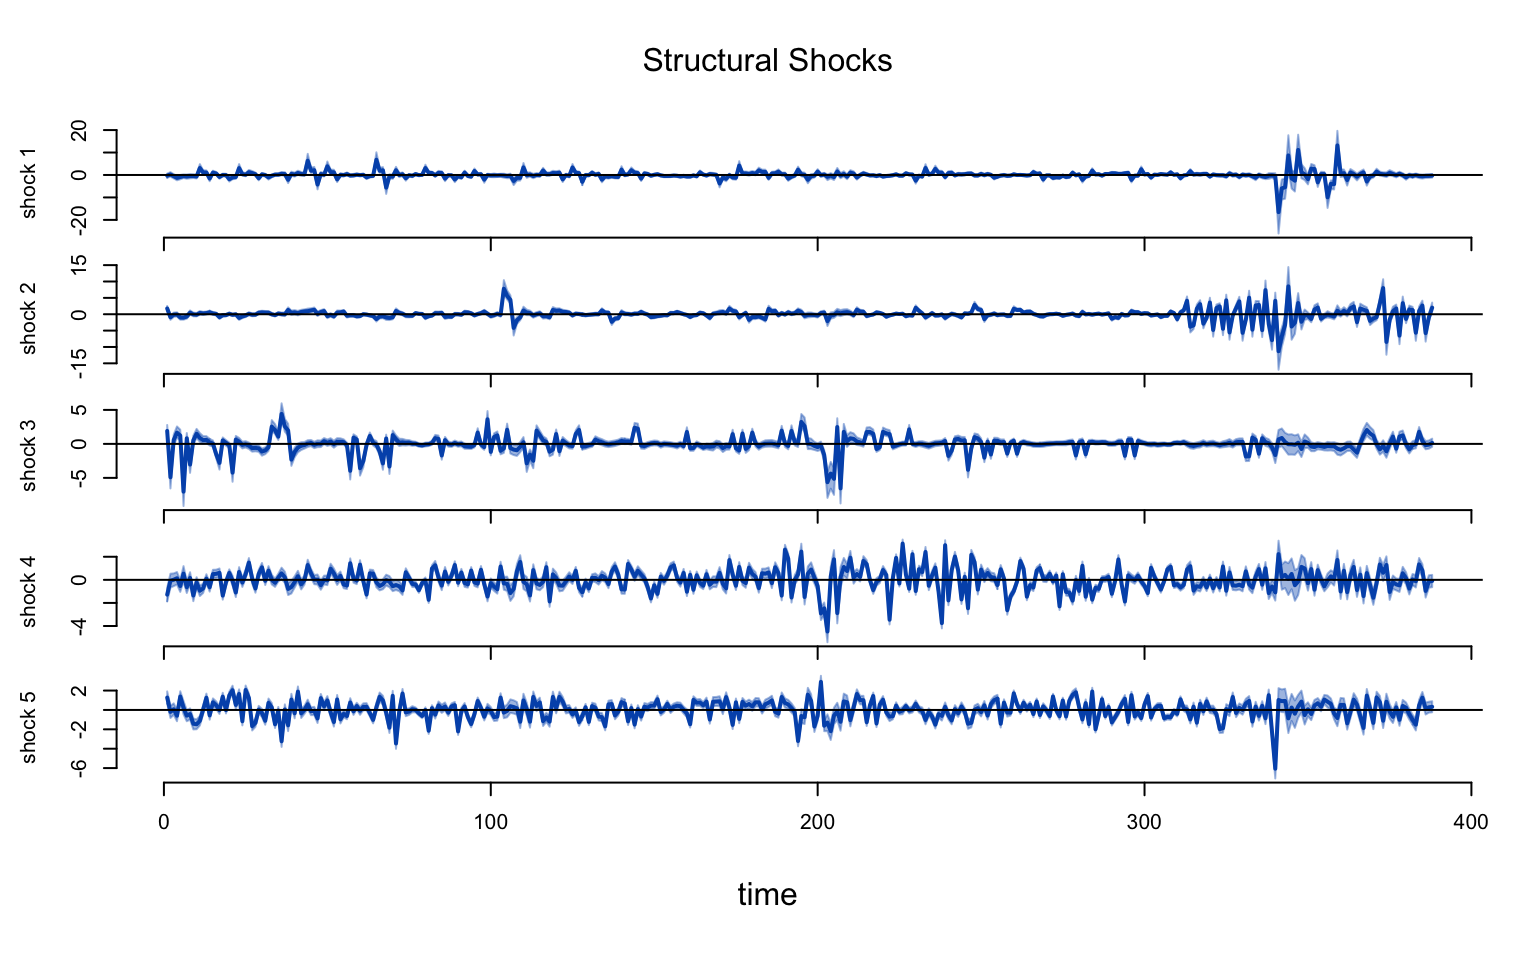
\includegraphics[scale=0.25]{bs_ss}
	\end{frame}
	

	
	\begin{frame}{\huge bsvars.org features}
		\centering
		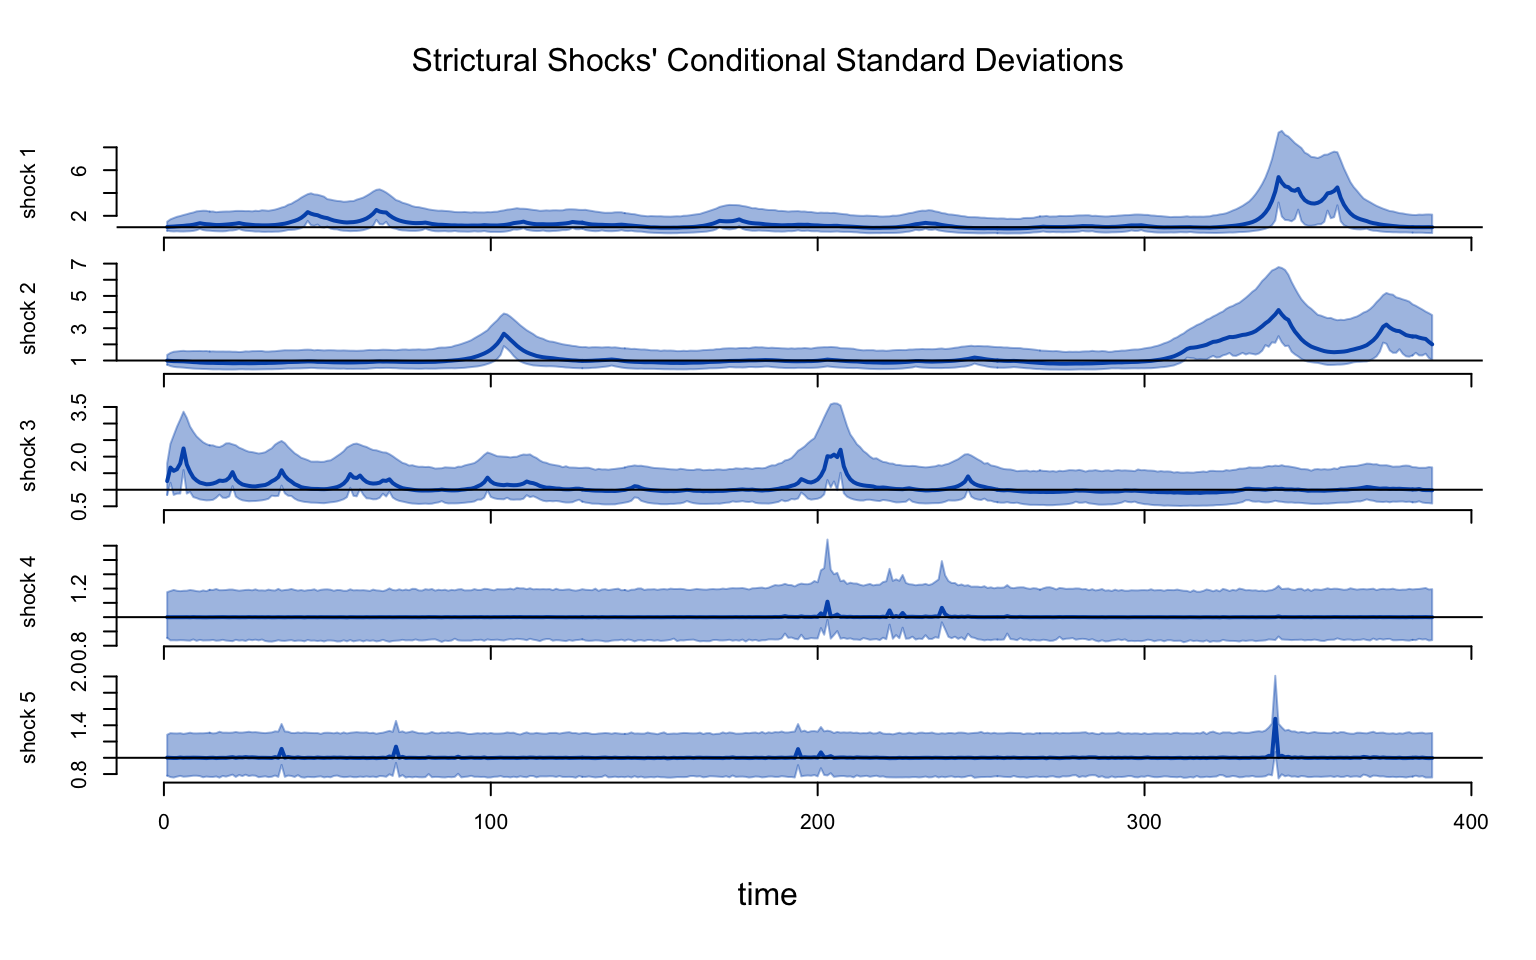
\includegraphics[scale=0.25]{bs_sds}
	\end{frame}
	
	
	\begin{frame}{\huge bsvars.org features}
		\centering
		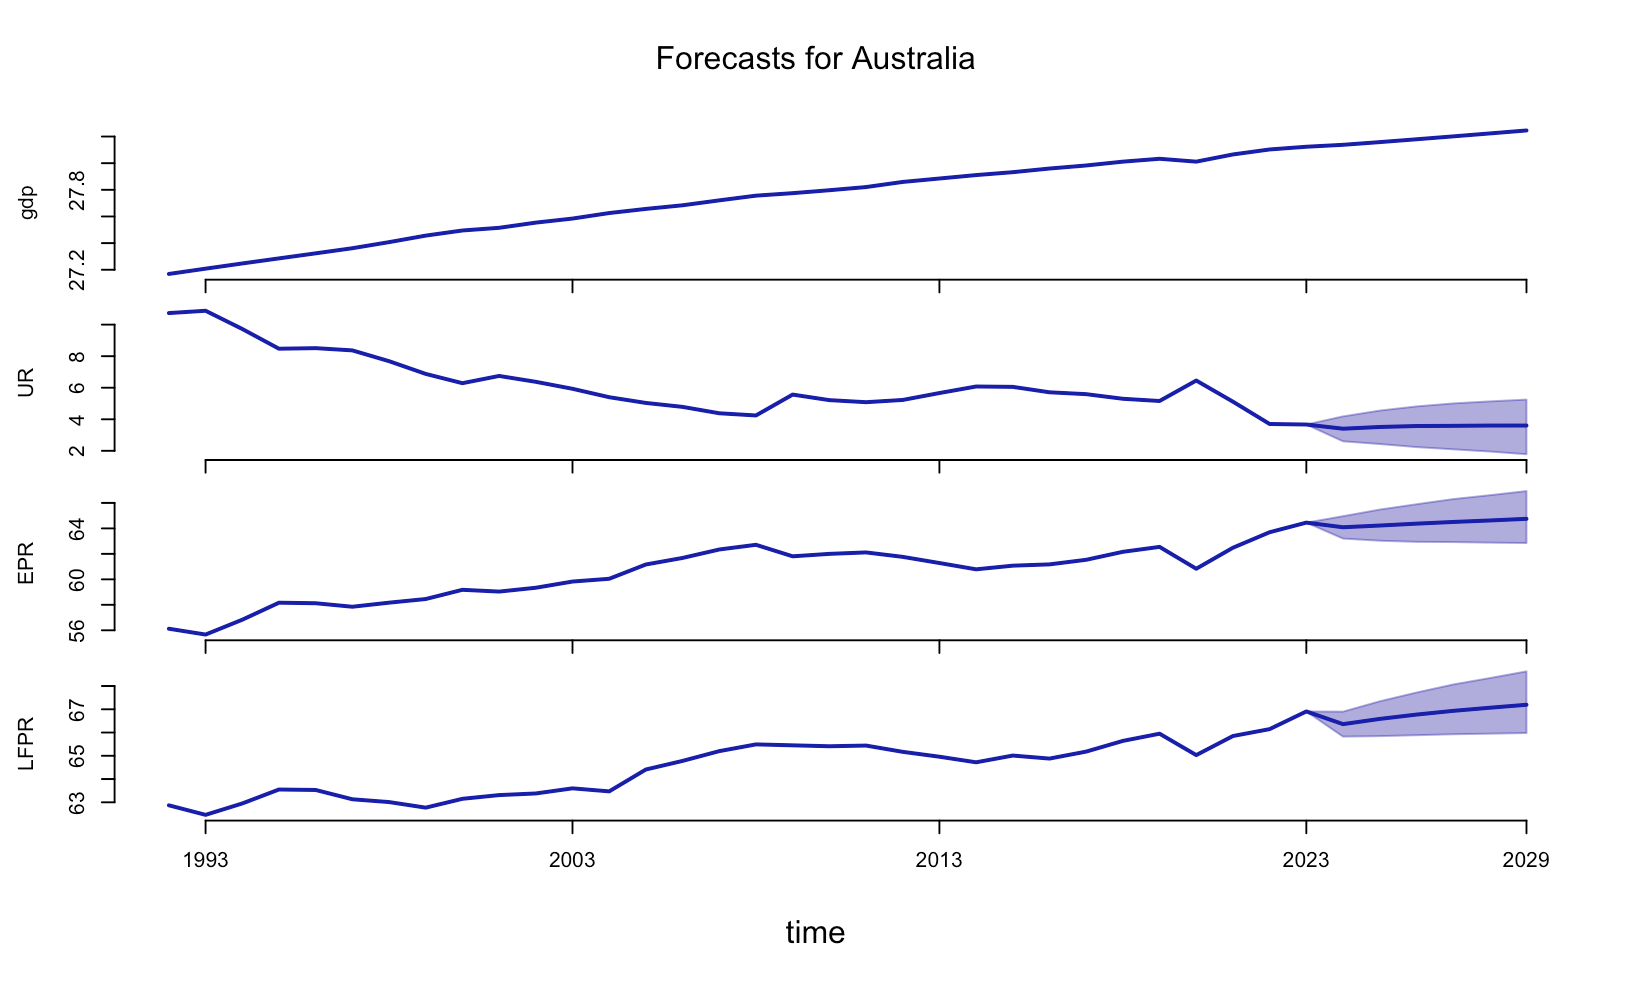
\includegraphics[scale=0.5]{bs_fore}
	\end{frame}

	
	
	\begin{frame}{\huge bsvars.org roadmap}
		\Large
		
		\begin{itemize}[label=$\blacktriangleright$]
		{\color{lig}
			\item R package \textbf{bvarPANELs}\\[0.5ex]
			Forecasting with Bayesian Hierarchical Panel VARs\\[1ex]
			\item R package \textbf{bsvarTVPs} \\[0.5ex]
			Bayesian SVARs with Time-Varying Identification\\[1ex]
			\item R package \textbf{bsvarCFs}\\[0.5ex]
			Conditional Forecasting for Bayesian Structural VARs
		}	
		\end{itemize}
	\end{frame}


	
	
	
	
	
	
	
	
	
		
	{\setbeamercolor{background canvas}{bg=lig}
		\begin{frame}
			\centering
			
\includegraphics[scale=0.3]{social}
		\end{frame}
	}
	


\end{document} 
